
% \vspace{-.8in}
%% {\centering
%% \hspace{.68in}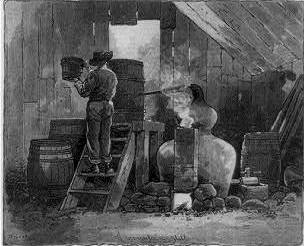
\includegraphics[width=.6\textwidth]{../pictures/moonshine.jpg}\par
%% }

%% \subsubsection{Peering into Learning}

%% \noindent This is a quick introduction to the main ideas used in the rest of the
%% book. It provides a range of things to think about as you get started
%% with a new peer learning project, or as you use peeragogy to redesign
%% and reassess an existing collaboration. You'll probably want to read
%% this first and then do some reflection before diving into the other
%% parts of the book.

\subsubsection{Motivation}
\noindent You might wonder why we're doing this project -- what we
hope to get out of it as volunteers, and how we think what we're doing
can make a positive difference in the world. Have a look at this
chapter if you, too, are thinking about getting involved in peeragogy,
or wondering how peeragogy can help you accelerate your learning
projects.

\paragraph{\emph{Case Study: 5PH1NX.}}
This example focuses on the interrelationship of pedagogy and
peeragogy in a high school English class, when students are
encouraged to find and share creative ways to learn. Explore this
case study for ideas and encouragement for your own learning
adventures.

\subsubsection{Peeragogy in Practice}

\noindent Here we describe some of the interaction patterns that we've
encountered time and time again in the Peeragogy project.  You can use
the ideas in this chapter as a starter-kit for your own experiments
with peeragogy right away.  Sharing -- and revising -- patterns is one
of the key activities in peeragogy, so you will likely want to revisit
this chapter several times as you look through the rest of the book.
Don't forget your red pen or pencil, because you'll also want to
tailor the patterns we describe here to suit.

\paragraph{\emph{Case Study: SWATS.}}
We present another example of peer learning in a classroom setting,
focusing on the process of improving overall student performance with
the help of a group of student experts.  After describing the case
study in general terms, we then re-analyze it using our pattern tools
to show how examples like this can be integrated into our project.

\subsubsection{Convening a Group}

\noindent This chapter is about how to begin your own peeragogical project.
You can also use the ideas described here to strengthen an existing
collaboration.  Simple but important questions will inspire unique
answers for you and your group.  In short: who, what, when, where,
why, and how?  Use this chapter to help design and critique your
project's roadmap.

 \paragraph{\emph{Play \& Learning.}} What
makes learning fun? Just as actors learn their roles through the dynamic
process of performance, In other words, the more we engage with a topic,
the better we learn it and the more satisfying - or fun - the process
becomes.

\paragraph{\emph{K-12 Peeragogy.}} The key to becoming a successful
`connected educator-learner' involves spending the time needed to learn
how to learn and share in an open, connected environment. Once you make
the decision to enter into a dialogue with another user, you become a
connected educator/learner and tap into the power of networks to
distribute the load of learning. Depending on their age, you can even
facilitate an awareness of peer networks among your students.

\paragraph{\emph{P2P Self-Organizing Learning Environments.}} This
section engages invites an exploration of support for self-organized
learning in global and local networks.  Emergent structures
can create startling ripple effects.

\subsubsection{Organizing a Learning Context}

\noindent Peer learning is sometimes organized in ``courses'' and
sometimes in ``spaces.''  We present the results of an informal poll
that reveals some of the positive and some of the negative features of
our own early choices in this project.

\paragraph{\emph{Adding Structure with Activities.}} The first rule of thumb for
peer learning is: announce activities only when you plan to take part
as a fully engaged participant. Then ask a series of questions: what
is the goal, what makes it challenging, what worked in other
situations, what recipe is appropriate, what is different about
learning about this topic?

\paragraph{\emph{Student Authored Syllabus.}}  This chapter
describes various methods for co-creating a curriculum.  If you're
tasked with teaching an existing curriculum, you may want to start
with a smaller co-created activity; but watch out, you may find that
co-creation is habit forming.\footnote{Quick tip: if you create a
syllabus, share it!}

\paragraph{\emph{Case Study: Collaborative Explorations.}} This
chapter describes collaborative peer learning among adult students in
the Master's program in Critical and Creative Thinking at University
of Massachusetts in Boston.  The idea in the collaborative
explorations is to encourage individuals pursuing their own interests
related to a predetermined topic, while supporting learning of
everyone in the group through sharing and reflection.  These
interactions of supportive mutual inquiry evolve the content and
structure within a short time frame and with open-ended results.

\subsubsection{Cooperation}

\noindent Sometimes omitting the figurehead empowers a group.
Co-facilitation tends to work in groups of people who gather to share
common problems and experiences. The chapter suggests several ways to
co-facilitate discussions, wiki workflows, and live online sessions.
Conducting an ``after action review'' can help expose blind spots.

\paragraph{\emph{The Workscape.}} In a corporate workscape, people are free-range
learners: protect the learning environment, provide nutrients for
growth, and let nature take its course. A workscape features profiles,
an activity stream, wikis, virtual meetings, blogs, bookmarks, mobile
access and a social network.

\paragraph{\emph{Participation.}} Participation grows from having a
community of people who learn together, using a curriculum as a starting
point to organize and trigger engagement. Keep in mind that
participation may follow the 90/9/1 principle (lurkers/editors/authors)
and that people may transition through these roles over time.

\paragraph{\emph{Designs For Co-Working.}}
Designing a co-working platform to include significant peer learning
aspects often requires a new approach.  This chapter describes the
initial steps of converting an existing online encyclopedia project
into a peer learning platform.

\subsubsection{Assessment}

\noindent  ``Usefulness'' is an appropriate
metric for assessment in peeragogy, where we're concerned with
devising our own problems rathan than the problems that have been
handed down by society.  We use the idea of return on investment (the
value of changes in behavior divided by the cost of inducing the
change) to assess the Peeragogy project itself, as one example.

\paragraph{\emph{Researching peeragogy.}} This chapter is based on a ``found manuscript'' created by one of us as an undergraduate.  It looks at the
challenges that are associated with combining the roles of student,
teacher, and researcher.  It shows the relevance of peer support, and
also illustrates the important factor of time in the evolution of an
idea.

\subsubsection{Technologies, Services, and Platforms}

\noindent Issues of utility, choice, coaching, impact and roles attach
to the wide variety of tools and technologies available for peer
learning. Keys to selection include the features you need, what people
are already using, and the type of tool (low threshold, wide wall,
high ceilings) used for collaboration.

\paragraph{\emph{Forums.}} Forums are web-based communication media
that enable groups of people to conduct organized multimedia discussions
about multiple topics over a period of time, asynchronously. A rubric
for evaluating forum posts highlights the value of drawing connections.
The chapter includes tips on selecting forum software.

\paragraph{\emph{Wiki.}} A
wiki is a website whose users can add, modify, or delete its content via
a web browser. Pages have a feature called ``history'' which allows
users to see previous versions and roll back to them. The chapter
includes tips on how to use a wiki and select a wiki engine, with
particular attention to peer learning opportunities.

 \paragraph{\emph{Real-time meetings.}} Web services enable broadband-connected
learners to communicate in real time via audio, video, slides,
whiteboards, chat, and screen-sharing. Possible roles for participants
in real-time meetings include searchers, contextualizers, summarizers,
lexicographers, mappers, and curators. This mode of interaction
supports emergent agendas.

\paragraph{\emph{Connectivism in Practice.}} Massive Open
Online Courses (MOOCs) are decentralized online learning experiences:
individuals and groups create blogs or wikis and comment on each
other's work, often with other tools helping find information.

\subsubsection{Resources}

\noindent Here we present a sample syllabus for bringing peer learning
to life, recommended reading and tips on writing for The Handbook, as
well as our Creative Commons Zero 1.0 Universal (CC0 1.0) Public
Domain Dedication.
